\documentclass{article}

\usepackage{fancyhdr}
\usepackage{extramarks}
\usepackage{amsmath}
\usepackage{amsthm}
\usepackage{tikz}
\usepackage{enumerate}
\usepackage{comment}

\usetikzlibrary{automata, positioning}

\topmargin=-0.45in
\evensidemargin=0in
\oddsidemargin=0in
\textwidth=6.5in
\textheight=9.0in
\headsep=0.25in

\linespread{1.1}

\pagestyle{fancy}
\lhead{\hmwkAuthorName\ -\ \hmwkAuthorID}
\chead{\hmwkClass: Homework \hmwkNo}
\rhead{\firstxmark}
\lfoot{\lastxmark}
\cfoot{\thepage}

\renewcommand\headrulewidth{0.4pt}
\renewcommand\footrulewidth{0.4pt}

\newcommand{\enterProblemHeader}[1]{
    \nobreak\extramarks{}{Problem \arabic{#1} continued on next page\ldots}\nobreak{}
    \nobreak\extramarks{Problem \arabic{#1} (continued)}{Problem \arabic{#1} continued on next page\ldots}\nobreak{}
}

\newcommand{\exitProblemHeader}[1]{
    \nobreak\extramarks{Problem \arabic{#1} (continued)}{Problem \arabic{#1} continued on next page\ldots}\nobreak{}
    \stepcounter{#1}
    \nobreak\extramarks{Problem \arabic{#1}}{}\nobreak{}
}

\setcounter{secnumdepth}{0}
\newcounter{homeworkProblemCounter}
\setcounter{homeworkProblemCounter}{1}
\nobreak\extramarks{Problem \arabic{homeworkProblemCounter}}{}\nobreak{}

\newenvironment{homeworkProblem}[1][-1]{
    \ifnum#1>0
        \setcounter{homeworkProblemCounter}{#1}
    \fi
    \section{Problem \arabic{homeworkProblemCounter}}
    \enterProblemHeader{homeworkProblemCounter}
}{
    \exitProblemHeader{homeworkProblemCounter}
}


\newenvironment{solution}{
    \subsection{Solution}
}

\newcommand{\hmwkNo}{1}
\newcommand{\hmwkDueDate}{Sunday, March 17, 2019 at 11:59pm}
\newcommand{\hmwkClass}{CS244 Theory of Computation}
\newcommand{\hmwkClassInstructor}{Fu Song}
\newcommand{\hmwkAuthorName}{Yuyang Rong}
\newcommand{\hmwkAuthorID}{69850764}

\title{
    \vspace{-0.4in}
    \textmd{\textbf{\hmwkClass \\ Homework \hmwkNo}}\\
    \normalsize\vspace{0.1in}\small{Due: \hmwkDueDate}\\
}

\author{\hmwkAuthorName\ -\ \hmwkAuthorID}
\date{}

\begin{document}

\maketitle
\thispagestyle{fancy}

You may discuss this assignment with other students and work
on the problems together. However, your write-up should be your own individual work and you should indicate in your submission who you worked with, if applicable. You should use the {\LaTeX} template provided by us to write your solution and submit the generated PDF file into Gradescope. \\

I worked with: (Name, ID), (Name, ID), \ldots \\

Let $\Sigma = \{\mathsf{0}, \mathsf{1}\}$ if not otherwise specified.

\begin{homeworkProblem}
Let $A$ be the set of all strings where there are no consecutive $\mathsf{0}$'s. Show that $A$ is regular in the following ways:
\begin{enumerate}[(a)]
    \item by giving an $\mathsf{NFA}$ that recognizes $A$,
    \item by giving a $\mathsf{DFA}$ that recognizes $A$,
    \item by giving a regular expression that describes $A$, and
    \item by giving a right linear grammar that describes $A$.
\end{enumerate}

\begin{solution}
\subsubsection{a)}
	Since DFA is a subset of NFA, we would skip NFA part and draw a DFA as respond to both a) and b).
\subsubsection{b)}
	\begin{center}
	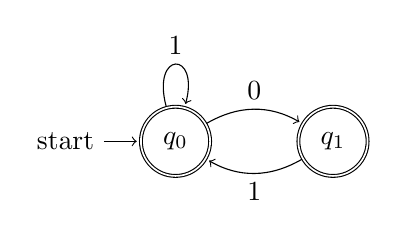
\begin{tikzpicture}[shorten >=1pt,node distance=2cm,on grid,auto]
		\node[state, initial, accepting] 	(q_0) 					{$q_0$};
		\node[state, accepting] 			(q_1) 	[right=of q_0] 	{$q_1$};
		\path[->]
			(q_0) 	edge 	[loop above] 	node 	{1} 	()
					edge 	[bend left]		node 	{0} 	(q_1)
			(q_1) 	edge 	[bend left]		node 	{1} 	(q_0);
	\end{tikzpicture}
	\end{center}
\subsubsection{c)}
	\[
		L = 1^*(01^+)^*
	\]
\subsubsection{d)}
	$$ G = (\mathcal{N}, \Sigma, \mathcal{P}, \mathcal{S}) \texttt{ s.t. } \mathcal{N}=\{\mathcal{S}, A, B\}, \Sigma = \{0, 1\}, \mathcal{P} \texttt{ consists of the following rules: } $$
	\begin{equation*}\begin{aligned}
		& \mathcal{S} \rightarrow AB \\
		& A \rightarrow 1A | \epsilon \\
		& B \rightarrow 01A | \epsilon
	\end{aligned}\end{equation*}
\end{solution}

\end{homeworkProblem}

\begin{homeworkProblem}
Let $B$ be the set of all strings with even length that contain at least one $\mathsf{1}$ in their first half.
\begin{enumerate}[(a)]
    \item Show that $B$ is not regular.
    \item Show that $B$ is context free.
\end{enumerate}
\begin{solution}
\subsubsection{a)}
	\begin{proof}
		Let's proof by contradiction: Suppose $B$ is regular, is must satisfy pumping lemma, then $\exists p \ge 1$ \\
		Now consider string $0^{2p-1}10^{2p} \in B$. \\
		To satisify condition 3: $|xy| \le q$, it is safe to say that $x=0^s$, $y=0^t$ and $t > 0$ and $s + t \le p$. \\
		Then $\forall i$, $xy^i=0^{s+ti}$, $xy^iz = 0^{s+ti+(2p-1-s-t)}10^{2p}$. \\
		To fail condition 1, we can have $xy^i$ long enough to fail condition ``at least one $\mathsf{1}$ in the first half'' and formulate the following equation:
		\begin{equation*}\begin{aligned}
			 |xy^i| &\ge \frac{1}{2}(|xy^iz|) \\
			 s + it &\ge \frac{1}{2}(s + ti + 2p-1-s-t + 1 + 2p) \\
			 i 		&\ge \frac{1}{t}(4p-2s-t) > 1
		\end{aligned}\end{equation*}
		Therefore, $\forall i \ge \frac{1}{t}(4p-2s-t)$, condition 1 cannot stand, this contradicts to pumping lemma which claims that $\forall i$, condition 1 stand. \\
		Therefore, we  claim that $B$ is not regular.
	\end{proof}
\subsubsection{b)}
	\begin{proof}
		We can proof that $B$ is context free by constructing a CFG that accepts $B$. Now, consider 
		$$(\mathcal{N}, \Sigma, \mathcal{P}, \mathcal{S})$$
		$$\mathcal{N} = \{\mathcal{S}, \texttt{Any}\}$$
		Now we can descirbe $\mathcal{P}$ as following:
		\begin{equation*}\begin{aligned}
			& \mathcal{S} \rightarrow 1 \texttt{Any} 0 | 1 \texttt{Any} 1 | 0\mathcal{S}0 | 0\mathcal{S}1\\
			& \texttt{Any} \rightarrow 1 \texttt{Any} 0 | 1 \texttt{Any} 1 | 0 \texttt{Any} 0 | 0 \texttt{Any} 1 |\epsilon
	\end{aligned}\end{equation*}
	\end{proof}
\end{solution}
\end{homeworkProblem}

\begin{homeworkProblem}
Show that the following languages are not regular. B refers to the language in Problem 2.
\begin{enumerate}[(a)]
    \item $C = \{w \mid w \in B \text{ or } w \text{ has odd length}\}$.
    \item $D = \{w \mid w \text{ has even length but } w \notin B\}$.
\end{enumerate}
\end{homeworkProblem}
\begin{solution}
\subsubsection{a)}
	\begin{proof}
		Let's proof by contradiction. \\
		Suppose C is regular. Then using closure properities we have: \\
		$$B = C \cap \{w | w \texttt{ has even length}\}$$
		Since $C$ and $\{w | w \texttt{ has even length}\}$ is regular, this implies that B is regular, which contradicts to the fact that $B$ is not regular.
	\end{proof}
\subsubsection{b)}
	\begin{proof}
		Let's rephrase $D$ first. $D = \{lr | l=0^k, r = \Sigma^k\}$, that is to say, $\forall s \in D$, there is no $\mathsf{1}$ in the fist half $s$
		\\
		We would be proofing that $D$ is not regular by using Myhill-Nerode Theorem. \\
		Consider an infinite array of strings: $s_k = 0^k1, k = 1, 2, 3, \cdots$, we would be proving that they are not equivalent to each other w.s.t. $\~_L$ \\
		\\
		$\forall i \ne j$, without loss of generation, let's assume $i > j$. \\
		Then we can construct a $u = 1^j$ s.t. $s_ju \in D$ yet $s_iu \notin D$ \\
		\\
		Therefore, we proved that $D$ is not regular by proving that $D$ has a equivalent class that has infinite size.
	\end{proof}
\end{solution}

\begin{homeworkProblem}
For any string $w = w_1 w_2 \dotso w_n$, the \emph{reverse} of $w$, written as $w^\mathcal{R}$, is the string $w$ in reverse order, $w_n \dotso w_2 w_1$. For any language $A$, let $A^\mathcal{R} = \{w^\mathcal{R} \mid w \in A\}$. Show that if $A$ is regular, so is $A^\mathcal{R}$, i.e., regular languages are closed under reversal.
\end{homeworkProblem}
\begin{proof}
	We would be proving by constructing an NFA that accepts $A^\mathcal{R}$. \\
	\\
	Since $A$ is regular, there must be a DFA $(Q, \Sigma, \delta, q_0, F)$ that accepts $A$.
	To accept $A^\mathcal{R}$, we reverse the original DFA and construct the following NFA:
	$$(Q\cup\{q_0'\}, \Sigma, \delta', q_0', q_0)$$
	where we have $q_0'$ as start state, the original $q_0$ is now accept state. \\
	We also change the definition of $\delta'$:
	$$\forall q \in Q, \alpha \in \Sigma, \delta(q, \alpha) = q_{next}\texttt{, we define } \delta'(q_{next}, \alpha) = \{q\} $$
	$$\texttt{Also, } \delta'(q_0', \epsilon) = F$$
\end{proof}

\begin{homeworkProblem}
Consider the following $\mathsf{CFG}\ G$:
$$S \to \mathsf{0} S \mathsf{1} \mid \mathsf{00} S \mathsf{1} \mid \varepsilon$$
Describe $L(G)$ and show that $G$ is ambiguous. Give an unambiguous grammar $H$ where $L(H) = L(G)$ and sketch a proof that $H$ is unambiguous.
\end{homeworkProblem}
\begin{solution}
\subsubsection{a)}
	$$L(G) = \{0^i1^j | i=x+y, j=x+2y\}$$
\subsubsection{b)}
	Consider Grammar $H = (\mathcal{N}, \Sigma, \mathcal{P}, \mathcal{S})$, $\mathcal{N} = \{\mathcal{S}, \texttt{M}, \texttt{U}\}$
	Now we can descirbe $\mathcal{P}$ as following:
	\begin{equation*}\begin{aligned}
		& \mathcal{S} \rightarrow \texttt{M} | \texttt{U} \\
		& \texttt{M} \rightarrow 0 \texttt{M} 1 | \epsilon \\
		& \texttt{U} \rightarrow 00\texttt{U}1 | 00\texttt{M}1
	\end{aligned}\end{equation*}
\end{solution}

\begin{homeworkProblem}
Let $E = \{rst \mid r, t \in \mathsf{0}^* \text{ and } s \in \mathsf{0}^* \mathsf{1} \mathsf{0}^* \text{ where } |r| = |s| = |t|\}$. Show that $E$ is context free in two ways:
\begin{enumerate}[(a)]
    \item by giving a $\mathsf{CFG}$ that generates $E$, and
    \item by giving a $\mathsf{PDA}$ that recognizes $E$.
\end{enumerate}
\end{homeworkProblem}
\begin{solution}
\subsubsection{a)}
	Consider grammar $G=(\mathcal{N}, \Sigma, \mathcal{P}, \mathcal{S})$, $\mathcal{N} = \{\mathcal{S}\}$
	Now we can descirbe $\mathcal{P}$ as following:
	\begin{equation*}\begin{aligned}
		& \mathcal{S} \rightarrow 00S0 | 0S00 | 010 \\
	\end{aligned}\end{equation*}
\subsubsection{b)}
	Consider $M=(\{q\}, \Sigma, \Sigma\cup \mathcal{N}, \delta, q, \mathcal{S}, \emptyset)$, we define $\delta$ as follow:
	\begin{equation*}\begin{aligned}
		& \delta(q, \epsilon, S) =  \{(q, 010), (q, 00S0), (q, 0S00)\} \\
		& \delta(q, 0, 0) = \{(q, \epsilon)\} \\
		& \delta(q, 1, 1) = \{(q, \epsilon)\}
	\end{aligned}\end{equation*}	

\end{solution}

\begin{homeworkProblem}
Let $F = \{rst \mid r, s, t \in \mathsf{0}^* \mathsf{1} \mathsf{0}^* \text{ where } |r| = |s| = |t|\}$.
\begin{enumerate}[(a)]
    \item Show that $F$ is not context free.
    \item Is $F \cup (\Sigma \Sigma \Sigma)^*$ context free? Prove your answer.
    \item Is $F \cup \Sigma (\Sigma \Sigma \Sigma)^*$ context free? Prove your answer.
\end{enumerate}
\end{homeworkProblem}
\subsubsection{a)}
	\begin{proof}
		We would be showing that $F$ is not context free using contradiction. \\
		Suppose $F$ is context free, $F$ satisfies pumping lemma. \\
		Then consider string: $uvwxy = 0^{p}110^{p}10^{p}$ \\
		\\
		\textbf{Condition1}: 
			$1 \in v \texttt{ or } 1 \in x$. \\
			In this case $\forall i > 2, uv^iwx^iy \notin F$, as $\forall s \in F$, only 3 $1$s will be present. \\
		\\
		\textbf{Condition2}: 
			$1 \notin v \texttt{ and } 1 \notin x$, i.e. $v = 0^a, x = 0^b, a+b \equiv 0 (mod 3)$ \\
			We have to assume that $\exists k > 0, a+b = 3k$, or else the string will not have a total length of $3n$ when pumping. \\	
			We also point out that $v$ or $x$ cannot have part of it in $r$ and part of it in $s$, or it must contain $1$. \\
			\\
			\textbf{Condition2.1}: First let's argue that $v$ substring $s$ and $x$ substring $t$ is impossible\\
				If $v$ substring $s$ and $x$ substring $t$, consier $\forall a > 0, b>0, i>0$, the string $uv^iwx^iy = 0^p110^{p-a+ia}1p^{p-b+ib}$ \\
				Now consider the first one third half, aka, its $r$. We can be assured that $$|r| = \frac{3p + 3 + (i-1)(a+b)}{3} = p+1+(i-1)k > p+1$$
				Therefore $r = 0^p110^{(i-1)k-1}$. There are two $1$s in $r$.
				So we come to the conclusion that $v$ substring $s$ and $x$ substring $t$ is impossible \\ 
			\\
			\textbf{Condition2.2}: We also need to proof that $v$ substring $r$ and $x$ substring $t$ is impossible. \\
			If so, $|vwx| \le p$ cannot be satisfied. It is impossible for $v$ substring $r$ while $x$ substring $t$.\\
			\\
			\textbf{Condition2.3}: 
				$v$ substring $r$ and $x$ substring $t$. \\
				In this case, we would have: 
				$$uv^ixy^iz = 0^{p-a+ia}110^{p-b+bi}10^{p} = 0^{p-(i-1)a}110^{p-(i-1)b}10^{p}$$
				$$|r| = p+1+(i-1)k$$
				To help with our discussion we further divide the cases based on the relation of $a$ and $b$\\
			\\
			\textbf{Conditition2.3.1} $2a > b \Rightarrow a > k$ \\
				If $a>k$, we consider when $i > \frac{1}{a-k}$: \\
				Since $i > \frac{1}{a-k}$, \\
				we have $p+1+(i-1)k < p+(i-1)a$, further:
				$r = 0^{p+1+(i-1)k}$, having no $1$ in it. \\
				This partition is impossible. 
			\\
			\textbf{Conditition2.3.2} $2a < b \Rightarrow a < k$ \\
				In this case, consider when $i > \frac{1}{k-a} + 1$:
				Since $i > \frac{1}{k-a} + 1$, \\
				we have $p+1+(i-1)k > p+2+(i-1)a$, fruther: 
				$|r| = p+1+(i-1)k \Rightarrow r = 0^{p+(i-1)a}110^{(i-1)(k-a)-1}$.\\
				This means that there are 2 $1$s in $r$, so it is not possible. \\
			\textbf{Conditition2.3.3} $2a = b \Rightarrow a = k$ \\
				In this case, consider the case when $i = 0$, \\
				$|r| = p+1-k < p + 1$, $r = 0^{p+1-k}$, which has no $1$ inside, so it is also impossible.
		\\ \\
		\textbf{Therefore we have prove that for string $0^{p}110^{p}10^{p}$, there is no partition that satisfies pumping lemma, which implies $F$ is not context free.}

	\end{proof}

\subsubsection{b)}
	It is a context free grammar.
	\begin{proof}
		It is trivial that $F \subset (\Sigma\Sigma\Sigma)^* \Rightarrow F \cup (\Sigma \Sigma \Sigma)^* = (\Sigma \Sigma \Sigma)^*$ \\
		Therefore, the job become proving $(\Sigma \Sigma \Sigma)^*$ is context free, which again, is trivial.\\
		Since $(\Sigma \Sigma \Sigma)^*$ is a regular language, it must be context free since regular language is a subset of context free language.
	\end{proof}
\subsubsection{c)}
	It is not a context free grammar.
	\begin{proof}
		We would proof by contradiction: suppose it is CFG. \\
		Then construct regular language $T = (\Sigma\Sigma\Sigma)^*$, since CFG is closed under intersection with regular language, we have:\\
		$(F\cup\Sigma(\Sigma\Sigma\Sigma)^*) \cap T = F$ being CFG, which contradicts our conclusion in a).
	\end{proof}
\end{document}